% !TEX root = ../main.tex
\section{引言}

自然与社会中的许多复杂系统，都由大量相互作用的组分构成。
传染病在人群接触中传播，观点和信息沿社会关系扩散，物种通过捕食或竞争共同演化，
振荡单元借助耦合产生同步，
电力节点则通过输电网络彼此影响。
尽管这些系统的物理含义各不相同，
它们都可以抽象为“网络上的动力学”：节点描述组分及其状态，
边描述组分之间可能发生的作用，
状态随时间的变化则由自身规律与邻居影响共同决定\cite{strogatz2001,albert2002}。

理解这种演化过程具有直接的科学与应用意义。
一个可靠的动力学模型不仅应当回答“下一时刻会发生什么”，还应帮助我们解释哪些局部作用塑造了整体行为，
并支持更长时间的预测、风险评估与干预设计。
传统的正向研究通常从已知网络和已知方程出发：给定连接关系、动力学形式和参数，
计算系统从某个初态如何演化。
这一思路清晰而有效，
但其前提在现实中往往难以满足。

更常见的情形是，我们只能观测到各组分随时间变化的状态序列。
动力学方程可能不完整，关键参数需要从数据中估计，组分之间的真实连接甚至从未被记录。
于是问题由正向模拟转化为一个更困难的逆问题：能否从多变量时间序列中学习系统的演化规律？当网络不可见时，
能否进一步找回支撑这些规律的潜在连接？这两个问题分别对应动力学学习与网络拓扑重构，
也是把观测数据转化为可解释模型的关键步骤\cite{brunton2016,zhang2019ggn}。

这类逆问题的困难不只来自模型规模，还来自结构与动力学之间的耦合。
网络已知时，学习器需要区分“节点自身如何变化”和“邻居如何施加影响”；
若两类信息过早混合，
模型可能仍能完成一步预测，
却难以稳定地还原作用规律。
网络未知时，
结构和动力学还可能相互补偿：一张包含过多错误边的网络，
配合较弱的邻居响应，
也可能产生相近的短期预测。
因而，
仅凭分类准确率或单步损失，
无法判断模型是否真正学到了可信的演化机制与连接结构。

为了在可控条件下深入研究上述问题，本文选择复杂网络上的 SIR 传播过程作为代表性案例。
SIR 模型以易感、感染和康复三种状态刻画传播过程，
既是传染病建模的经典基础，
也可作为谣言、信息或创新扩散的简化原型\cite{kermack1927,pastorsatorras2015}。
它的规则简洁，
却同时包含状态依赖、非线性交互、随机转移和吸收态，
能够清楚检验学习器是否识别了邻居作用、是否恢复了动力学参数，
以及错误网络是否会被预测模型掩盖。
更重要的是，
本文使用的学习框架并不把 SIR 解析式写进模型；
替换节点状态编码、交互表示和输出形式后，
同一思路有潜力推广到其他网络动力学。

本文采用由简到繁的两阶段路线，如\cref{fig:pipeline}所示。
第一阶段假设网络已知，专注于如何从时间序列学习演化规律。
我们将节点自身状态与邻居交互分别编码，
在读出阶段再组合，
使模型能够分别使用自身演化和网络作用。
第二阶段移除已知网络这一条件，
引入可学习的离散拓扑生成器，
在候选网络和动力学规律之间交替优化，
并通过更具结构信息的样本组织与多初始化选择降低稠密补偿解的影响。
两阶段均同时考察一步预测、规律与参数诊断以及多步推演；
第二阶段额外评价具体边是否被正确恢复。

\begin{figure}[H]
  \centering
  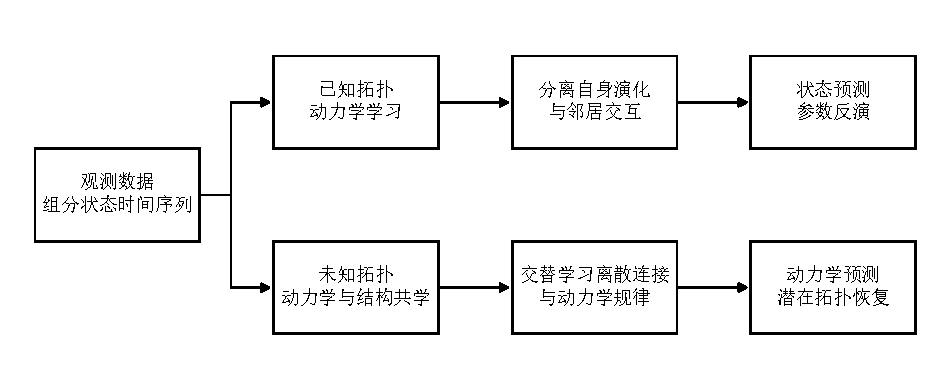
\includegraphics[width=\textwidth]{research_pipeline.pdf}
  \caption{本文研究路线。
相同的状态时间序列在网络已知与网络未知两种条件下形成递进任务：前者聚焦演化规律学习，后者进一步联合恢复潜在连接。
箭头仅表示信息与任务的推进关系。}
  \label{fig:pipeline}
\end{figure}

本文的主要工作包括以下三点。
\begin{enumerate}
  \item 提出一种面向网络动力学的自身--邻居双通道表示，将组分自身演化与邻居交互保持到读出阶段，以缓解量级失衡和表示混合，并通过多类图卷积对照分析其作用。
  \item 在网络不可见时，将离散拓扑生成与双通道动力学学习结合，通过硬图规律学习、软图结构更新和结构信息采样，构成从时间序列同时学习动力学与潜在网络的方法。
  \item 以 SIR 传播为可解释验证案例，从一步预测、参数反演、多步推演和边级恢复四个层面评价模型。
结果既展示了方法在三类网络上的有效性，
也揭示了联合学习仍可能出现的结构坍缩与适用边界。
\end{enumerate}

全文其余部分依次回顾数据驱动动力学学习、图神经网络与潜在关系推断的相关研究；
给出一般问题形式和 SIR 验证场景；
介绍已知与未知网络下的两阶段方法；
讨论实验结果、方法适用范围及向其他复杂系统动力学扩展的方向。
